\chapter{Overall Description}

\section{Product perspective}

The system will be developed from scratch and it will completely replace the legacy system. \newline

\vspace{0.8em}
\begin{figure}[H]
	\centering
	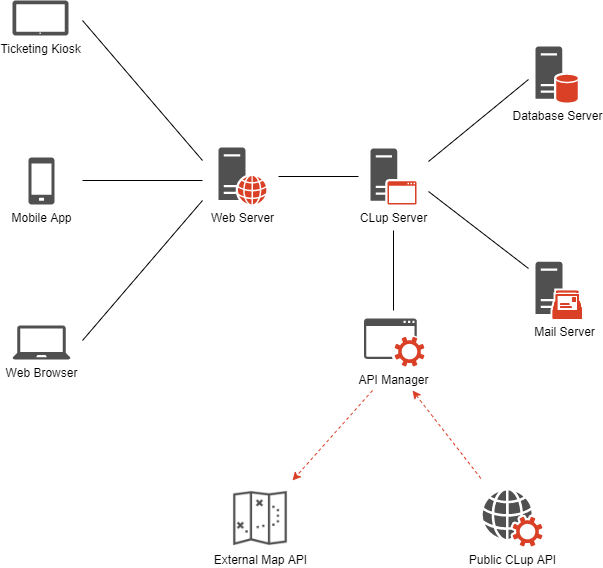
\includegraphics[scale=0.45]{product_perspective_diagram}
	\caption{CLup system diagram.}
\end{figure}


It is composed by a client part and a server part:
\begin{itemize}
	\item \textbf{Server side:}
	\begin{itemize}
		\item \textit{Application Server (CLup Server):} server where all the logic is located. It communicates with other servers and is the central point of the system.
		\item \textit{Web Server:} server used for the communication with the clients.
		\item \textit{Database Server:} server where all data are stored.
		\item \textit{Mail Server:} server used to send confirmation emails about the bookings.
		\item \textit{External map API:} API used to retrieve data about the distance of the user from the store. This information will be used to inform the user of when leave the current place.
	\end{itemize}
	\item \textbf{Client side:}
	\begin{itemize}
		\item \textit{User App:} Application installed on customers smartphone. It allows to retrieve a ticket or book a visit.
		\item \textit{Store App:} Application installed on employees smartphone. It allows to validate store passes.
		\item \textit{Ticketing Kiosk:} Tablet installed at the entrance of the store to which a printer is attached. It has installed a modified version of the mobile app which is able to print the ticket on place.
		\item \textit{Web Browser:} Used by store employees and managers to access the web dashboard.
	\end{itemize}
\end{itemize}

\subsection{Class diagram}

\begin{figure}[H]
	\centering
	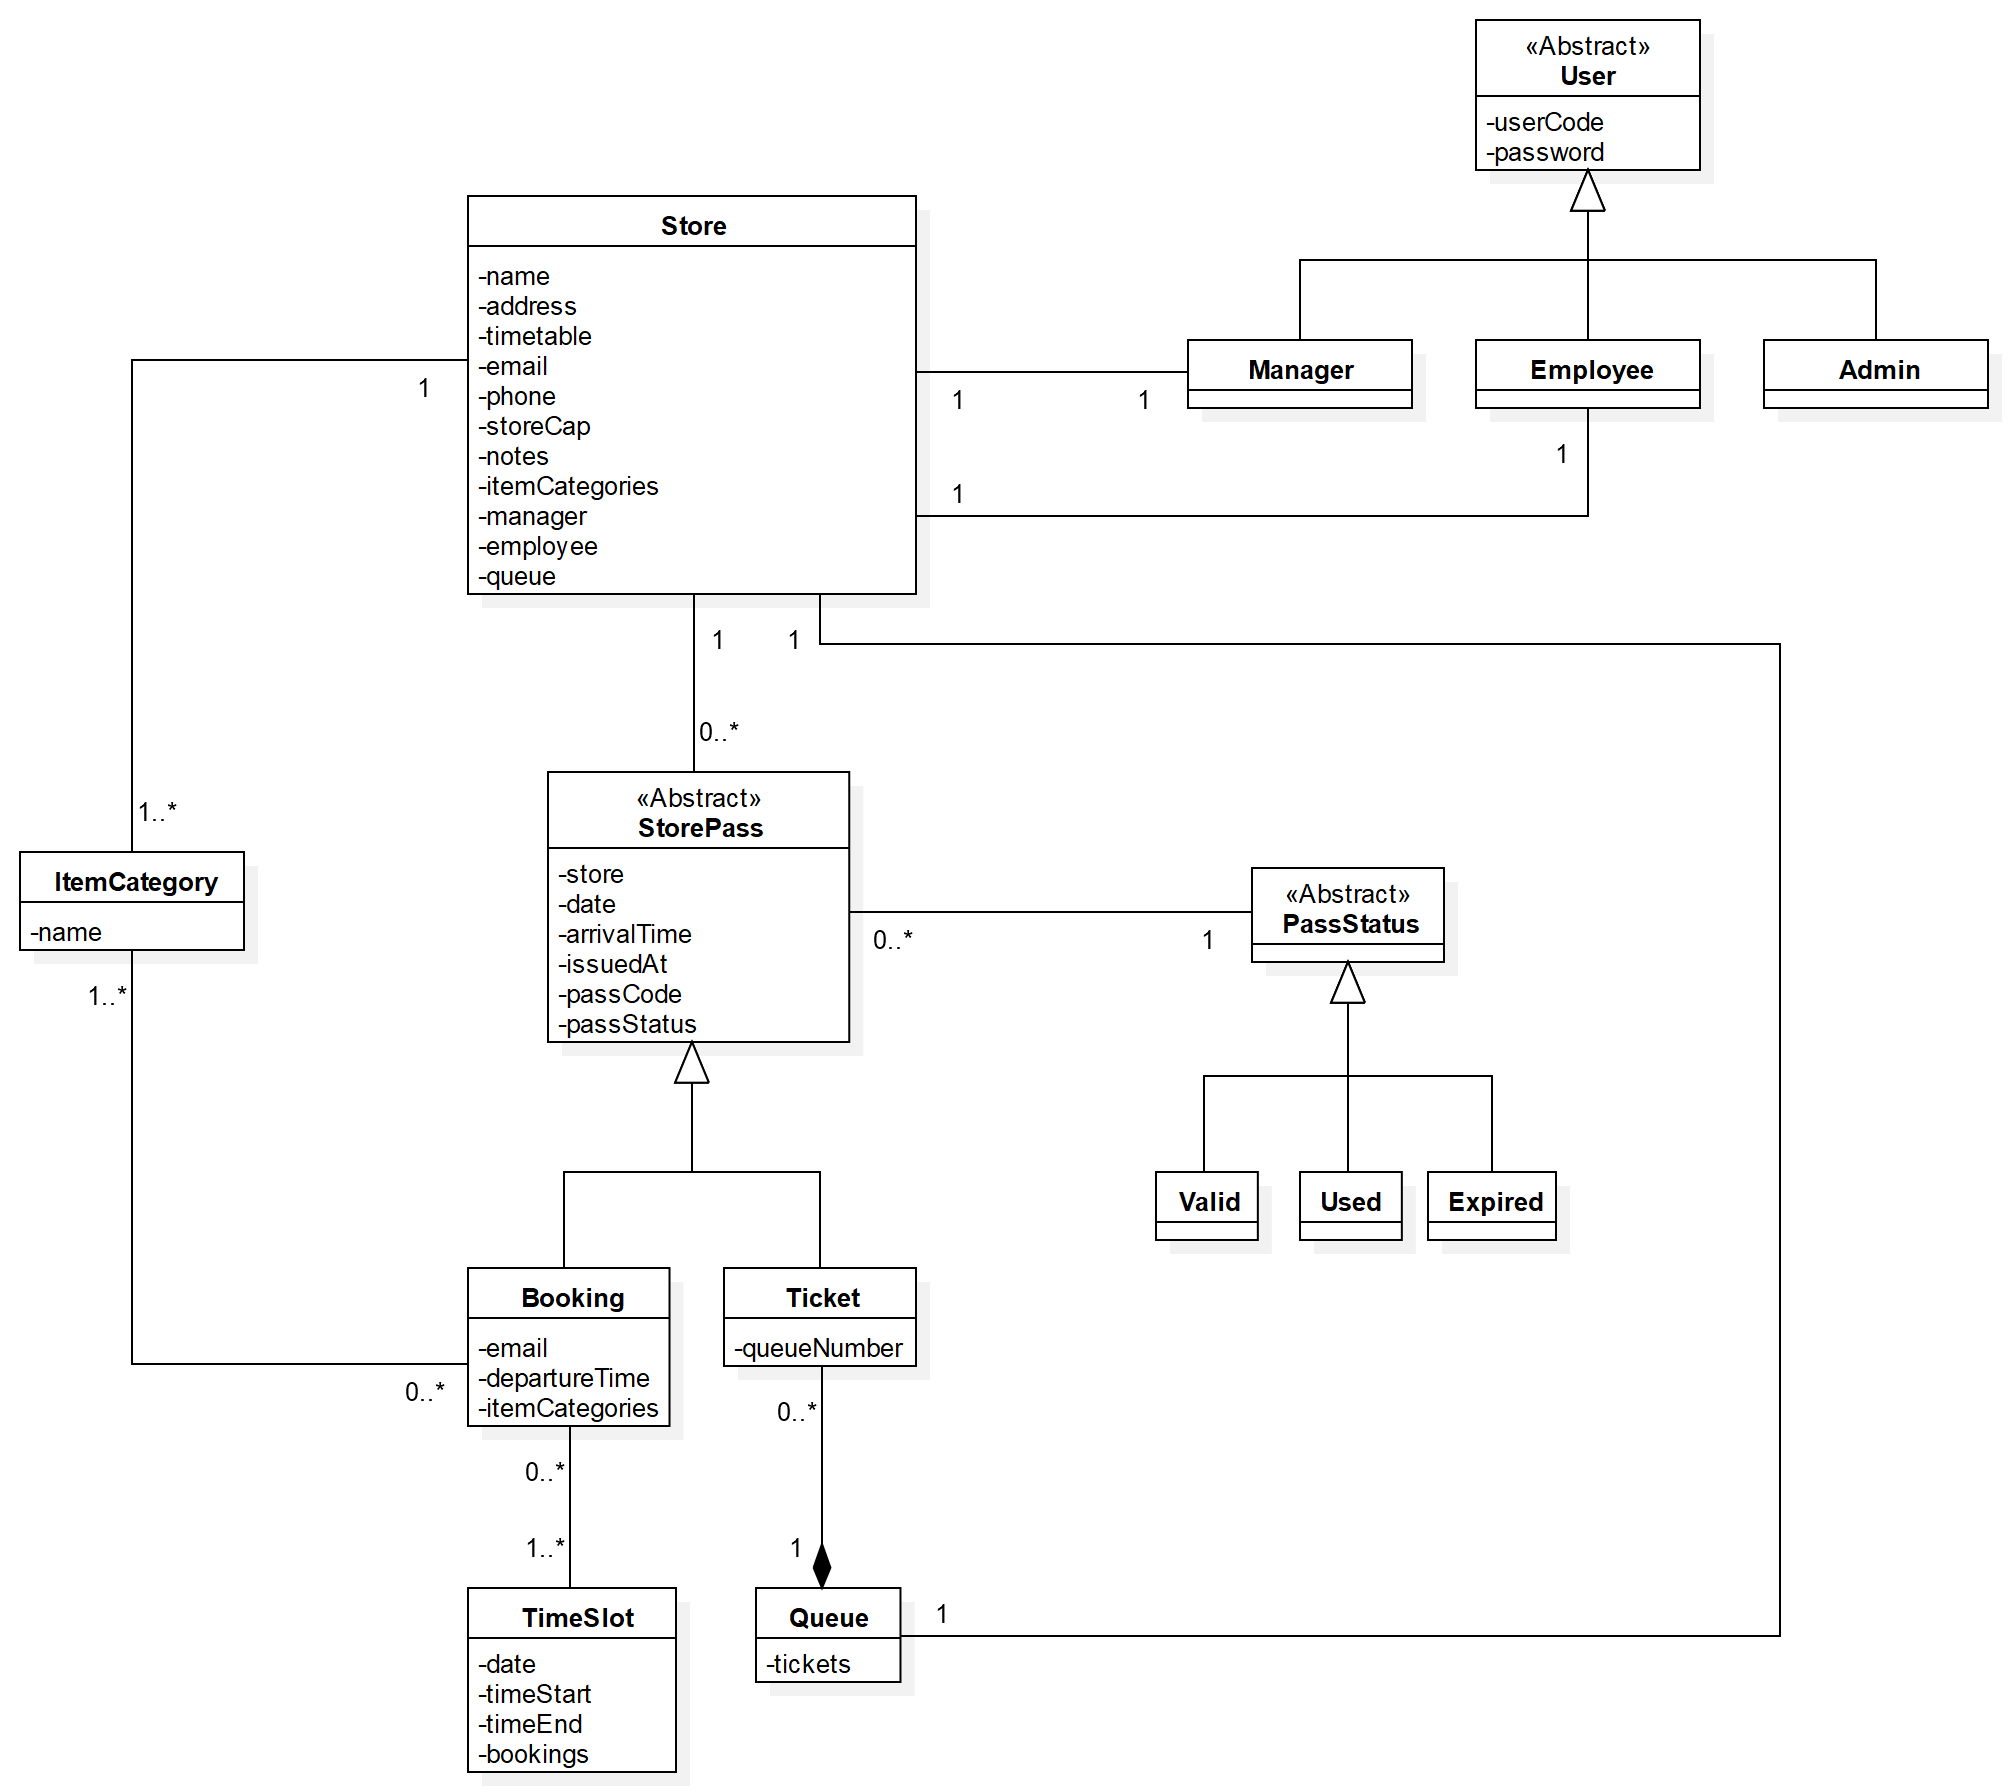
\includegraphics[width=\linewidth]{class_diagram}
	\caption{Class diagram.}
\end{figure}


\subsection{State diagrams}

\begin{figure}[H]
	\centering
	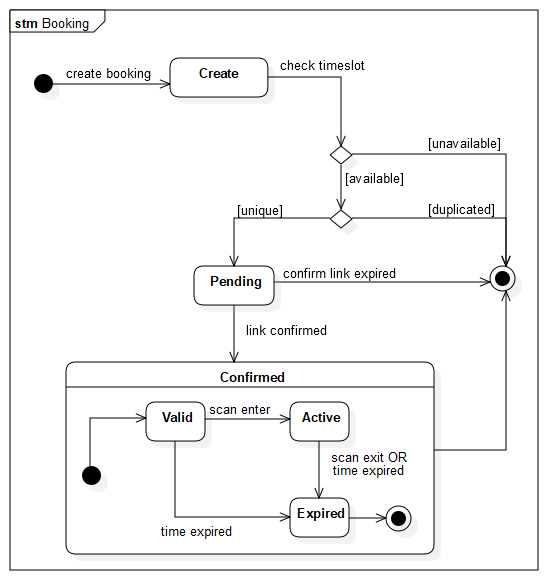
\includegraphics[width=\linewidth]{stm_booking}
	\caption{State diagram: Booking.}
\end{figure}

\begin{figure}[H]
	\centering
	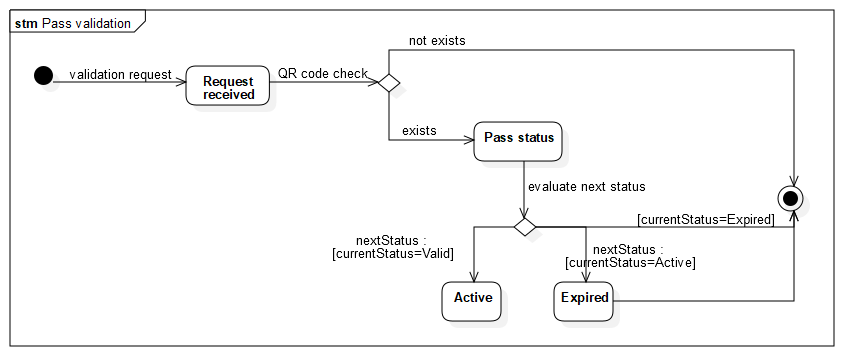
\includegraphics[width=\linewidth]{stm_pass_validation}
	\caption{State diagram: Pass validation.}
\end{figure}


\section{Product functions}\label{desc:prodFunc}
This section provides a summary of the major functions that the software will perform w.r.t. the goals already described in section \clupref{intro:goals}.

\subsection{Store pass function}
	A Store pass, among other things, consists of a QR code and a pass status. The latter identifies the current status inside the pass life-cycle:
	\begin{itemize}
		\item VALID: pass not used yet.
		\item ACTIVE: pass in use.
		\item EXPIRED: pass no longer acceptable. The period of time for which it could be used has ended or the pass has been successfully used.
	\end{itemize}

	The system also takes care of managing delays of customers: a delay greater than 15 minutes will result in the expiration of the pass. This implies that the customer will not be able to enter the store with that pass, instead they shall create a new one.\newline
	Among the available store seats, about the 15\% of them are reserved only for the bookings.
	
	Note that to benefit from these functions, the GPS service on customers' smartphones must be enabled, otherwise the application will not work.

	\subsubsection{Queue function}
	The main function of \textit{CLup} is to manage queues. A user who wants to do grocery-shopping will join the queue for a specific store through the User App.\newline
	
	Firstly, the user will be asked to select the store in which he desires to line-up.\newline
	Then the system will prompt the current size of the queue and an estimate of waiting time. If the user is satisfied with his choice it can subscribe to the queue upon completing a CAPTCHA. The operation will be confirmed by the emission of a ticket. The ticket comprehends a queue number, which identify user's position in the queue, and a QR code, which is used for the ticket validation.
	
	At any time the user will be able to check his position in the queue and the \textit{leave-at-time} (i.e. the time they need to depart from their current position to reach the store). When the user has to leave from where he is, the system sends a notification. The current position will be retrieved by the GPS of the user device.

	\subsubsection{Reserve function}
	This advanced function allows customers to "book a visit" to the store.
	A booking has an additional status attribute (i.e. booking status) which can be:
	\begin{itemize}
		\item PENDING: the booking has not been confirmed via email yet.
		\item CONFIRMED: the booking has been confirmed via email.
	\end{itemize}

	Customers are asked to select the store they want to visit. Then they need to fill in a form by indicating:
	\begin{itemize}
		\item an \textbf{email address}, which will be needed to send a receipt and memo to the user;
		\item the \textbf{date} of the visit;
		\item the approximate \textbf{expected duration} of the trip;
	 	\item the main \textbf{categories of items} they intend to buy;
	    \item a \textbf{time slot} chosen from the ones suggested by the system.
	\end{itemize}
	Every field of the form is mandatory, this means that the user must complete all of them, including the solution of a CAPTCHA, in order to submit the reservation.
	
	Customers will have to make reservations at least one day in advance.\newline
	The system will send an email with a confirmation link to the email address provided. To complete the booking process, the user must click the confirmation link within 24 hours from the time of subscription and in any case at least 1 hour before the chosen time slot. Users who fail to do so will have their booking expired.

	The time slots will be suggested according to the saturation of the grocery shelves. The system will try to balance the number of people in each section of the store.\newline
	Customers are also allowed to delete their booking at any time by going to the right section in the User App or by clicking the link sent via email after the reservation.
	Also this function support the \textit{leave-at-time} features, as described above in the Queue Function.

	In addition, for long-term customers, the app suggests a time inferred by the system based on an analysis of the previous visits.

\subsection{Validation function}
The Staff App provides an interface that allows to scan QR codes by using the smartphone camera. This process is required in order to validate store passes.\newline
Ticket validation allows to speed up the check-in process and to increase the number of people in the store. At the same time it helps staff to detect the authenticity of tickets brought to them.\newline
The scan of the QR code will be executed:
\begin{itemize}
	\item at the \textbf{entrance} by a dedicated store employee to control the influx at the store entrance.
	\item at the \textbf{exit} by the cashiers in order to notify the exit of customers from the store. In case any customer loses the QR code inside the store, the cashiers will use a backup QR code.
\end{itemize}

\subsection{Dashboard function}
\textit{Customers Line-up} web platform grants supermarkets a way to manage queues and customers inside their stores. In particular, \textbf{upon authentication}, it offers three level of access: \textit{manager-level} and \textit{staff-level} for supermarkets and \textit{admin-level} for CLup administrators.

\begin{itemize}
	\item \textbf{Manager level}\newline
	With the \textbf{dashboard UI}, store managers have access to tables and data visualizations of their customers visits and behaviours. In particular, they can monitor the number of people in the queue and the ones inside the store. Then, based on those data they can setup the maximum cap of people inside the store.\newline
	Store managers can view, edit and delete the list of reservations made by the customer.\newline
	Last but not least, they can inspect information about the booked visits at any given time.

	\item \textbf{Entrance-staff level}\newline
	A store employee is able to view data about the number of people in the queue and inside the building. This is needed during the validation of tickets when the check-in staff scans QR and allows customers inside the store.

    \item \textbf{Admin level}\newline
    An administrator of CLup is able to register new supermarkets and generate the respective credentials to access \textit{manager-level} and \textit{staff-level}.
\end{itemize}


\section{User characteristics}
CLup has four different groups of users:
\begin{itemize}
	\item \textbf{Customers}: they are customers of the supermarket. They can be of all ages and don't necessarily have experience with technology. They can also be elderly	people who don't have a smartphone at all. For this reason the system should be as easy to use as possible and should provide an alternative way to retrieve a ticket in addition to the mobile app.
	\item \textbf{Store managers}: they are the managers of the store. They manage the number of people who can access the store and can monitor the ones that are in the supermarket. It is reasonable to assume that they have at least a minimum experience with technology and the use of computer. For this reason the dashboard with all the information about customers will be accessible from a web browser.
	\item \textbf{Store employee}: they are the employees of the store. They validate the tickets at the entrance/exit of the store. They could not have experience with technology. For this reason the Store App and the dashboard have a simple interface and the interaction that they should have with them is reduced to the bare minimum.
    \item \textbf{CLup admin}: an operator of CLup able to login to the platform by using his special credentials. It can register supermarkets and generate their credentials. It can also maintain and update the system. Registration for this kind of users is forbidden and it has to be added directly during the system's installation process.
\end{itemize}

\section{Constraints}
In this topic it is put on paper a general description about considerations, boundaries and items that will limit the system's options.

\subsection{Regulatory policies}
The mobile application requests the user's permission in order to retrieve and use their position at runtime.\newline
The email addresses provided when booking through CLup will not be used for commercial purposes or given to third parties.\newline
The email addresses provided by the stores during the registration process must be PEC addresses identified by a Certification Authority.

\subsection{Hardware limitations}
Here is listed where CLup is available depending on the devices. Please note that not all devices are supported.
\begin{itemize}
	\item User App
		\begin{itemize}
			\item iPhones with iOS version 13.5 or above, phones running Android 6 (Marshmallow) or above;
			\item 2G/3G/4G connection or Wi-Fi available;
			\item GPS service.
		\end{itemize}
	
		\item Store App
		\begin{itemize}
			\item iPhones with iOS version 13.5 or above, phones running Android 6 (Marshmallow) or above;
			\item 2G/3G/4G connection or Wi-Fi available;
			\item Camera.
		\end{itemize}

	\item Web Dashboard
		\begin{itemize}
			\item modern web browser like Firefox, Chrome or Safari;
			\item internet connection available.
		\end{itemize}
\end{itemize}

\subsection{Interfaces to other applications}
The proper functioning of the app is strictly subordinated to an external map service which will be accessed via API. This is required to compute travel distance and time for a matrix of origins and destinations (i.e. customer and store position).

A failure in the above described service will translate into the inability to use CLup.

\clearpage

\section{Assumptions and Dependencies}
The properties that hold in the analysed world will be listed below.
\subsection{Domain assumptions}
\begin{enumerate}[label=\textbf{D.\arabic*}]
	\item \itemtext{dom:smartphone}{The majority of the customers has a smartphone with internet available.}
	\item \itemtext{dom:categories}{Customers attains to the declared categories of items.}
	\item \itemtext{dom:internetStores}{Stores have an internet contract.}
	\item \itemtext{dom:pecStores}{Stores have a PEC address.}
	\item \itemtext{dom:workingGps}{GPS modules of customers' smartphones are working properly.}
	\item \itemtext{dom:gpsPrecision}{The precision of the GPS modules of customers' smartphones is greater than twenty meters.}
	\item \itemtext{dom:bringSmartphone}{Customers bring with themselves the smartphone that they used to retrieve a ticket or reserve a time slot.}
    \item \itemtext{dom:oneToOneQr}{A ticket or a booked visit is associated with exactly one person.}
    \item \itemtext{dom:custEmail}{Customers who want to book-a-visit have an email address.}
	\item \itemtext{dom:uniqueName}{Stores have unique names.}
	\item \itemtext{dom:employeeEntrance}{Each store has an employee at the entrance which check-in people.}
	\item \itemtext{dom:empSmartphone}{Store employees have a supplied smartphone with camera.}
	\item \itemtext{dom:empCamera}{The cameras of employees' smartphone are working properly.}
	\item \itemtext{dom:storeRegistered}{Store managers have registered their stores in CLup.}
	\item \itemtext{dom:timeArrival}{Customers comply with the arrival time assigned by the mobile app.}
	\item \itemtext{dom:capStores}{Store managers know the maximum capacity of customers in the building.}
   	\item \itemtext{dom:storeKiosk}{Each store has a Self Service Ticketing Kiosk accessible.}
\end{enumerate}

